\documentclass[10pt,a4paper]{article}
\usepackage[utf8]{inputenc}
\usepackage[english]{babel}
\usepackage{amsmath}
\usepackage{amsfonts}
\usepackage{amssymb}
\usepackage{graphicx}
\usepackage{xcolor}
\usepackage{tikz}
\usetikzlibrary{positioning}
\author{Jonas Schulz}
\begin{document}
\hspace{-4cm}
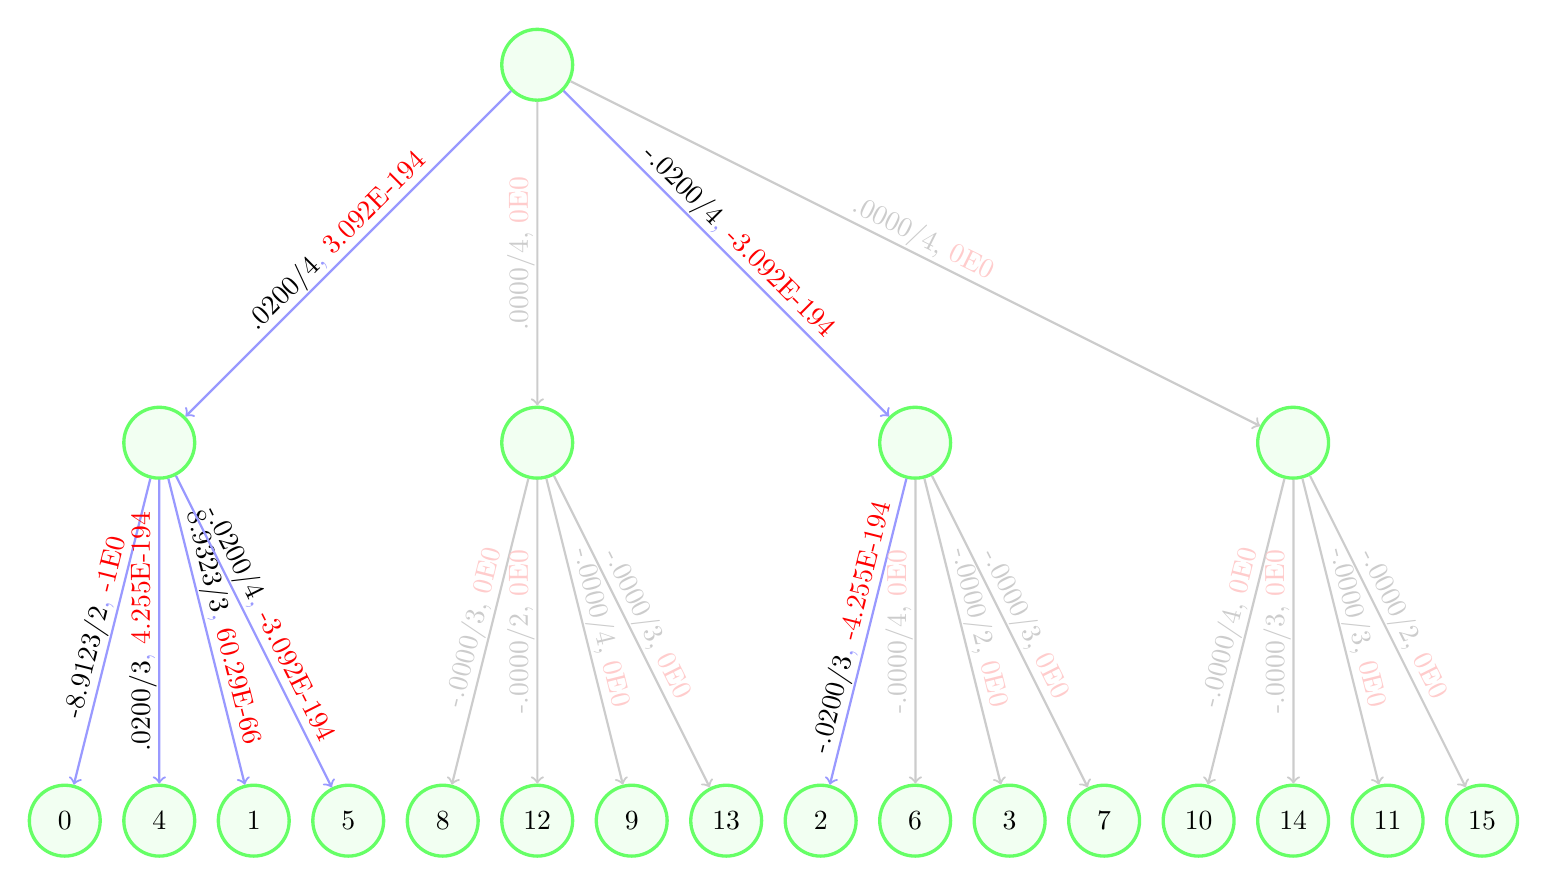
\begin{tikzpicture}[roundnode/.style={circle, draw=green!60, fill=green!5, very thick, minimum size=7mm}, scale=1.2]


\node[roundnode, minimum size = 0.9cm] at (8.0, 8) (0h8) {};
\node[roundnode, minimum size = 0.9cm] at (4.0, 4) (2h4) {};
\node[roundnode, minimum size = 0.9cm] at (3.0, 0) (2h0) {0};
\draw[thick, ->, color=blue!40] (2h4) -- (2h0) node[sloped,midway,above=-0.1cm] {\textcolor{black}{-8.9123/2}, \textcolor{red}{-1E0}};
\node[roundnode, minimum size = 0.9cm] at (4.0, 0) (3h0) {4};
\draw[thick, ->, color=blue!40] (2h4) -- (3h0) node[sloped,midway,above=-0.1cm] {\textcolor{black}{.0200/3}, \textcolor{red}{4.255E-194}};
\node[roundnode, minimum size = 0.9cm] at (5.0, 0) (4h0) {1};
\draw[thick, ->, color=blue!40] (2h4) -- (4h0) node[sloped,midway,above=-0.1cm] {\textcolor{black}{8.9323/3}, \textcolor{red}{60.29E-66}};
\node[roundnode, minimum size = 0.9cm] at (6.0, 0) (5h0) {5};
\draw[thick, ->, color=blue!40] (2h4) -- (5h0) node[sloped,midway,above=-0.1cm] {\textcolor{black}{-.0200/4}, \textcolor{red}{-3.092E-194}};
\draw[thick, ->, color=blue!40] (0h8) -- (2h4) node[sloped,midway,above=-0.1cm] {\textcolor{black}{.0200/4}, \textcolor{red}{3.092E-194}};
\node[roundnode, minimum size = 0.9cm] at (8.0, 4) (6h4) {};
\node[roundnode, minimum size = 0.9cm] at (7.0, 0) (6h0) {8};
\draw[thick, ->, color=black!20] (6h4) -- (6h0) node[sloped,midway,above=-0.1cm] {\textcolor{black!20}{-.0000/3}, \textcolor{red!20}{0E0}};
\node[roundnode, minimum size = 0.9cm] at (8.0, 0) (7h0) {12};
\draw[thick, ->, color=black!20] (6h4) -- (7h0) node[sloped,midway,above=-0.1cm] {\textcolor{black!20}{-.0000/2}, \textcolor{red!20}{0E0}};
\node[roundnode, minimum size = 0.9cm] at (9.0, 0) (8h0) {9};
\draw[thick, ->, color=black!20] (6h4) -- (8h0) node[sloped,midway,above=-0.1cm] {\textcolor{black!20}{-.0000/4}, \textcolor{red!20}{0E0}};
\node[roundnode, minimum size = 0.9cm] at (10.0, 0) (9h0) {13};
\draw[thick, ->, color=black!20] (6h4) -- (9h0) node[sloped,midway,above=-0.1cm] {\textcolor{black!20}{-.0000/3}, \textcolor{red!20}{0E0}};
\draw[thick, ->, color=black!20] (0h8) -- (6h4) node[sloped,midway,above=-0.1cm] {\textcolor{black!20}{.0000/4}, \textcolor{red!20}{0E0}};
\node[roundnode, minimum size = 0.9cm] at (12.0, 4) (10h4) {};
\node[roundnode, minimum size = 0.9cm] at (11.0, 0) (10h0) {2};
\draw[thick, ->, color=blue!40] (10h4) -- (10h0) node[sloped,midway,above=-0.1cm] {\textcolor{black}{-.0200/3}, \textcolor{red}{-4.255E-194}};
\node[roundnode, minimum size = 0.9cm] at (12.0, 0) (11h0) {6};
\draw[thick, ->, color=black!20] (10h4) -- (11h0) node[sloped,midway,above=-0.1cm] {\textcolor{black!20}{-.0000/4}, \textcolor{red!20}{0E0}};
\node[roundnode, minimum size = 0.9cm] at (13.0, 0) (12h0) {3};
\draw[thick, ->, color=black!20] (10h4) -- (12h0) node[sloped,midway,above=-0.1cm] {\textcolor{black!20}{-.0000/2}, \textcolor{red!20}{0E0}};
\node[roundnode, minimum size = 0.9cm] at (14.0, 0) (13h0) {7};
\draw[thick, ->, color=black!20] (10h4) -- (13h0) node[sloped,midway,above=-0.1cm] {\textcolor{black!20}{-.0000/3}, \textcolor{red!20}{0E0}};
\draw[thick, ->, color=blue!40] (0h8) -- (10h4) node[sloped,midway,above=-0.1cm] {\textcolor{black}{-.0200/4}, \textcolor{red}{-3.092E-194}};
\node[roundnode, minimum size = 0.9cm] at (16.0, 4) (14h4) {};
\node[roundnode, minimum size = 0.9cm] at (15.0, 0) (14h0) {10};
\draw[thick, ->, color=black!20] (14h4) -- (14h0) node[sloped,midway,above=-0.1cm] {\textcolor{black!20}{-.0000/4}, \textcolor{red!20}{0E0}};
\node[roundnode, minimum size = 0.9cm] at (16.0, 0) (15h0) {14};
\draw[thick, ->, color=black!20] (14h4) -- (15h0) node[sloped,midway,above=-0.1cm] {\textcolor{black!20}{-.0000/3}, \textcolor{red!20}{0E0}};
\node[roundnode, minimum size = 0.9cm] at (17.0, 0) (16h0) {11};
\draw[thick, ->, color=black!20] (14h4) -- (16h0) node[sloped,midway,above=-0.1cm] {\textcolor{black!20}{-.0000/3}, \textcolor{red!20}{0E0}};
\node[roundnode, minimum size = 0.9cm] at (18.0, 0) (17h0) {15};
\draw[thick, ->, color=black!20] (14h4) -- (17h0) node[sloped,midway,above=-0.1cm] {\textcolor{black!20}{-.0000/2}, \textcolor{red!20}{0E0}};
\draw[thick, ->, color=black!20] (0h8) -- (14h4) node[sloped,midway,above=-0.1cm] {\textcolor{black!20}{.0000/4}, \textcolor{red!20}{0E0}};


\end{tikzpicture}\\\\
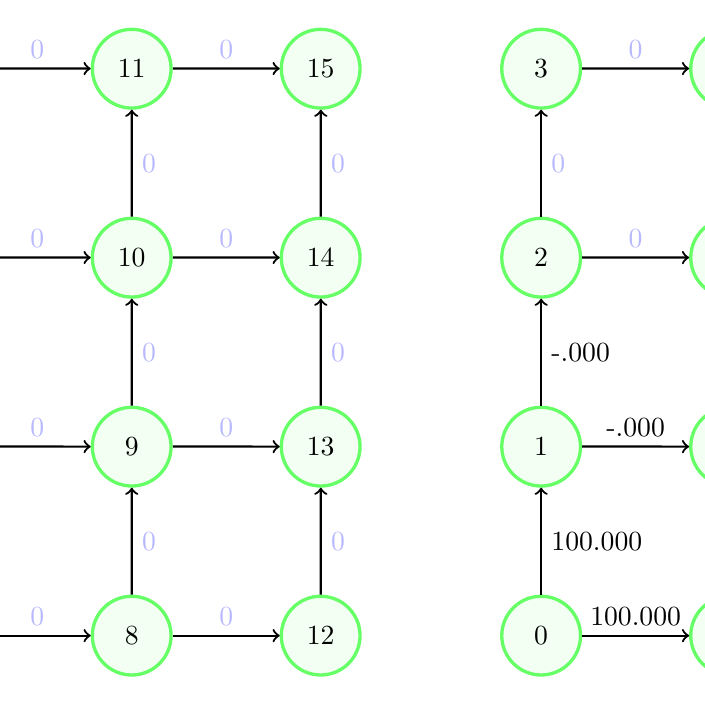
\begin{tikzpicture}[roundnode/.style={circle, draw=green!60, fill=green!5, very thick, minimum size=7mm}, scale=1.2]
\hspace{-4cm}

\node[roundnode, minimum size = 1cm] at (0.0, 0.0) (0) {\textcolor{black}{0}};
\node[roundnode, minimum size = 1cm] at (0.0, 2.0) (1) {\textcolor{black}{1}};
\node[roundnode, minimum size = 1cm] at (0.0, 4.0) (2) {\textcolor{black}{2}};
\node[roundnode, minimum size = 1cm] at (0.0, 6.0) (3) {\textcolor{black}{3}};
\node[roundnode, minimum size = 1cm] at (2.0, 0.0) (4) {\textcolor{black}{4}};
\node[roundnode, minimum size = 1cm] at (2.0, 2.0) (5) {\textcolor{black}{5}};
\node[roundnode, minimum size = 1cm] at (2.0, 4.0) (6) {\textcolor{black}{6}};
\node[roundnode, minimum size = 1cm] at (2.0, 6.0) (7) {\textcolor{black}{7}};
\node[roundnode, minimum size = 1cm] at (4.0, 0.0) (8) {\textcolor{black}{8}};
\node[roundnode, minimum size = 1cm] at (4.0, 2.0) (9) {\textcolor{black}{9}};
\node[roundnode, minimum size = 1cm] at (4.0, 4.0) (10) {\textcolor{black}{10}};
\node[roundnode, minimum size = 1cm] at (4.0, 6.0) (11) {\textcolor{black}{11}};
\node[roundnode, minimum size = 1cm] at (6.0, 0.0) (12) {\textcolor{black}{12}};
\node[roundnode, minimum size = 1cm] at (6.0, 2.0) (13) {\textcolor{black}{13}};
\node[roundnode, minimum size = 1cm] at (6.0, 4.0) (14) {\textcolor{black}{14}};
\node[roundnode, minimum size = 1cm] at (6.0, 6.0) (15) {\textcolor{black}{15}};
\draw[thick, ->] (0) -- (4) node[midway,above] {-.020};
\draw[thick, ->] (0) -- (1) node[midway,right] {-.020};
\draw[thick, ->] (1) -- (5) node[midway,above] {.020};
\draw[thick, ->] (1) -- (2) node[midway,right] {.020};
\draw[thick, ->] (2) -- (6) node[midway,above] {\textcolor{blue!28}{0}};
\draw[thick, ->] (2) -- (3) node[midway,right] {\textcolor{blue!28}{0}};
\draw[thick, ->] (3) -- (7) node[midway,above] {\textcolor{blue!28}{0}};
\draw[thick, ->] (4) -- (8) node[midway,above] {\textcolor{blue!28}{0}};
\draw[thick, ->] (4) -- (5) node[midway,right] {\textcolor{blue!28}{0}};
\draw[thick, ->] (5) -- (9) node[midway,above] {\textcolor{blue!28}{0}};
\draw[thick, ->] (5) -- (6) node[midway,right] {\textcolor{blue!28}{0}};
\draw[thick, ->] (6) -- (10) node[midway,above] {\textcolor{blue!28}{0}};
\draw[thick, ->] (6) -- (7) node[midway,right] {\textcolor{blue!28}{0}};
\draw[thick, ->] (7) -- (11) node[midway,above] {\textcolor{blue!28}{0}};
\draw[thick, ->] (8) -- (12) node[midway,above] {\textcolor{blue!28}{0}};
\draw[thick, ->] (8) -- (9) node[midway,right] {\textcolor{blue!28}{0}};
\draw[thick, ->] (9) -- (13) node[midway,above] {\textcolor{blue!28}{0}};
\draw[thick, ->] (9) -- (10) node[midway,right] {\textcolor{blue!28}{0}};
\draw[thick, ->] (10) -- (14) node[midway,above] {\textcolor{blue!28}{0}};
\draw[thick, ->] (10) -- (11) node[midway,right] {\textcolor{blue!28}{0}};
\draw[thick, ->] (11) -- (15) node[midway,above] {\textcolor{blue!28}{0}};
\draw[thick, ->] (12) -- (13) node[midway,right] {\textcolor{blue!28}{0}};
\draw[thick, ->] (13) -- (14) node[midway,right] {\textcolor{blue!28}{0}};
\draw[thick, ->] (14) -- (15) node[midway,right] {\textcolor{blue!28}{0}};




\hspace{10cm}


\node[roundnode, minimum size = 1cm] at (0.0, 0.0) (0) {\textcolor{black}{0}};
\node[roundnode, minimum size = 1cm] at (0.0, 2.0) (1) {\textcolor{black}{1}};
\node[roundnode, minimum size = 1cm] at (0.0, 4.0) (2) {\textcolor{black}{2}};
\node[roundnode, minimum size = 1cm] at (0.0, 6.0) (3) {\textcolor{black}{3}};
\node[roundnode, minimum size = 1cm] at (2.0, 0.0) (4) {\textcolor{black}{4}};
\node[roundnode, minimum size = 1cm] at (2.0, 2.0) (5) {\textcolor{black}{5}};
\node[roundnode, minimum size = 1cm] at (2.0, 4.0) (6) {\textcolor{black}{6}};
\node[roundnode, minimum size = 1cm] at (2.0, 6.0) (7) {\textcolor{black}{7}};
\node[roundnode, minimum size = 1cm] at (4.0, 0.0) (8) {\textcolor{black}{8}};
\node[roundnode, minimum size = 1cm] at (4.0, 2.0) (9) {\textcolor{black}{9}};
\node[roundnode, minimum size = 1cm] at (4.0, 4.0) (10) {\textcolor{black}{10}};
\node[roundnode, minimum size = 1cm] at (4.0, 6.0) (11) {\textcolor{black}{11}};
\node[roundnode, minimum size = 1cm] at (6.0, 0.0) (12) {\textcolor{black}{12}};
\node[roundnode, minimum size = 1cm] at (6.0, 2.0) (13) {\textcolor{black}{13}};
\node[roundnode, minimum size = 1cm] at (6.0, 4.0) (14) {\textcolor{black}{14}};
\node[roundnode, minimum size = 1cm] at (6.0, 6.0) (15) {\textcolor{black}{15}};
\draw[thick, ->] (0) -- (4) node[midway,above] {100.000};
\draw[thick, ->] (0) -- (1) node[midway,right] {100.000};
\draw[thick, ->] (1) -- (5) node[midway,above] {-.000};
\draw[thick, ->] (1) -- (2) node[midway,right] {-.000};
\draw[thick, ->] (2) -- (6) node[midway,above] {\textcolor{blue!28}{0}};
\draw[thick, ->] (2) -- (3) node[midway,right] {\textcolor{blue!28}{0}};
\draw[thick, ->] (3) -- (7) node[midway,above] {\textcolor{blue!28}{0}};
\draw[thick, ->] (4) -- (8) node[midway,above] {\textcolor{blue!28}{0}};
\draw[thick, ->] (4) -- (5) node[midway,right] {\textcolor{blue!28}{0}};
\draw[thick, ->] (5) -- (9) node[midway,above] {\textcolor{blue!28}{0}};
\draw[thick, ->] (5) -- (6) node[midway,right] {\textcolor{blue!28}{0}};
\draw[thick, ->] (6) -- (10) node[midway,above] {\textcolor{blue!28}{0}};
\draw[thick, ->] (6) -- (7) node[midway,right] {\textcolor{blue!28}{0}};
\draw[thick, ->] (7) -- (11) node[midway,above] {\textcolor{blue!28}{0}};
\draw[thick, ->] (8) -- (12) node[midway,above] {\textcolor{blue!28}{0}};
\draw[thick, ->] (8) -- (9) node[midway,right] {\textcolor{blue!28}{0}};
\draw[thick, ->] (9) -- (13) node[midway,above] {\textcolor{blue!28}{0}};
\draw[thick, ->] (9) -- (10) node[midway,right] {\textcolor{blue!28}{0}};
\draw[thick, ->] (10) -- (14) node[midway,above] {\textcolor{blue!28}{0}};
\draw[thick, ->] (10) -- (11) node[midway,right] {\textcolor{blue!28}{0}};
\draw[thick, ->] (11) -- (15) node[midway,above] {\textcolor{blue!28}{0}};
\draw[thick, ->] (12) -- (13) node[midway,right] {\textcolor{blue!28}{0}};
\draw[thick, ->] (13) -- (14) node[midway,right] {\textcolor{blue!28}{0}};
\draw[thick, ->] (14) -- (15) node[midway,right] {\textcolor{blue!28}{0}};


\end{tikzpicture}\\\\
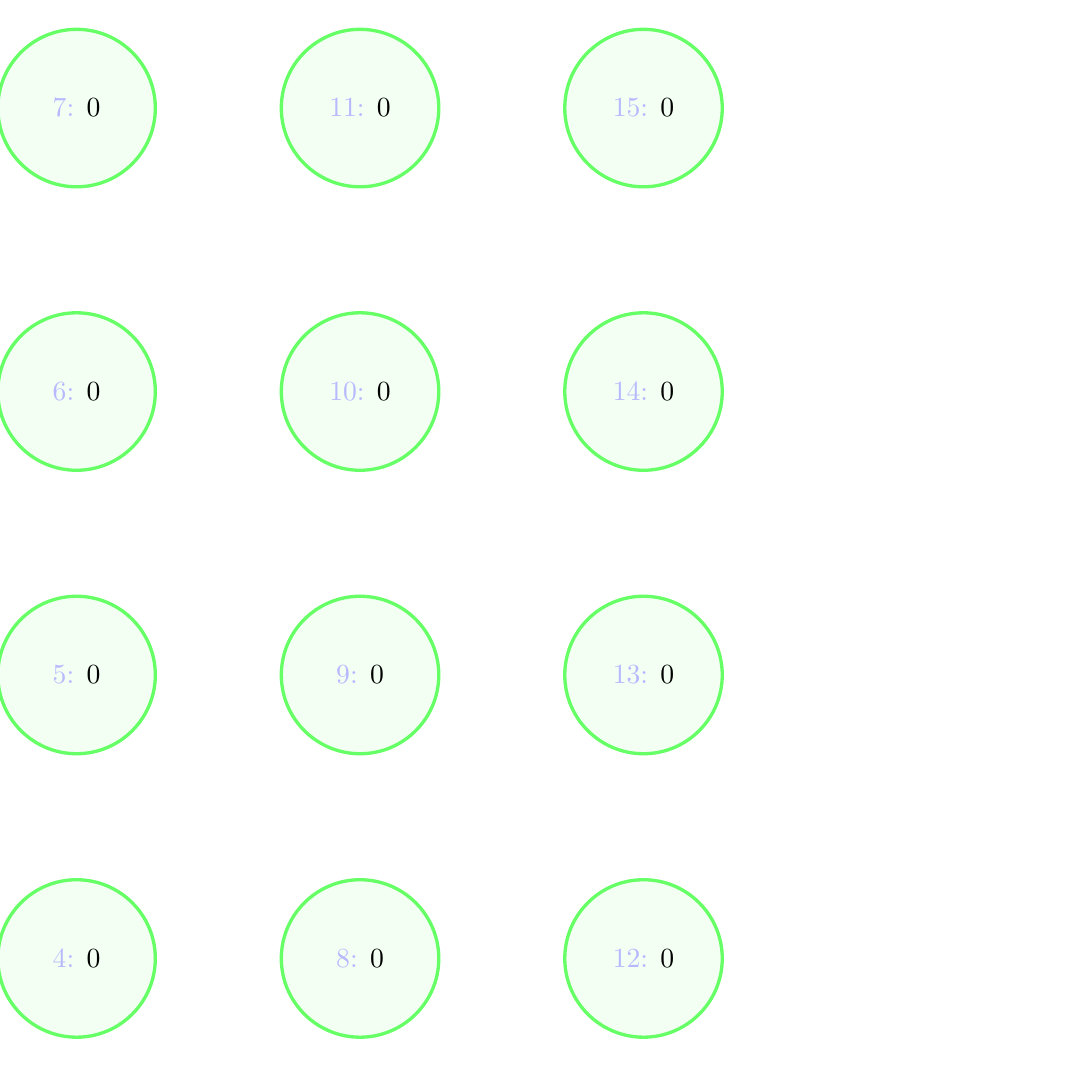
\begin{tikzpicture}[roundnode/.style={circle, draw=green!60, fill=green!5, very thick, minimum size=7mm}, scale=1.2]
\hspace{-4cm}

\node[roundnode, minimum size = 2cm] at (0.0, 0.0) {\textcolor{blue!28}{0:} \textcolor{red}{-8.872}};
\node[roundnode, minimum size = 2cm] at (0.0, 3.0) {\textcolor{blue!28}{1:} \textcolor{red}{8.872}};
\node[roundnode, minimum size = 2cm] at (0.0, 6.0) {\textcolor{blue!28}{2:} 0};
\node[roundnode, minimum size = 2cm] at (0.0, 9.0) {\textcolor{blue!28}{3:} 0};
\node[roundnode, minimum size = 2cm] at (3.0, 0.0) {\textcolor{blue!28}{4:} 0};
\node[roundnode, minimum size = 2cm] at (3.0, 3.0) {\textcolor{blue!28}{5:} 0};
\node[roundnode, minimum size = 2cm] at (3.0, 6.0) {\textcolor{blue!28}{6:} 0};
\node[roundnode, minimum size = 2cm] at (3.0, 9.0) {\textcolor{blue!28}{7:} 0};
\node[roundnode, minimum size = 2cm] at (6.0, 0.0) {\textcolor{blue!28}{8:} 0};
\node[roundnode, minimum size = 2cm] at (6.0, 3.0) {\textcolor{blue!28}{9:} 0};
\node[roundnode, minimum size = 2cm] at (6.0, 6.0) {\textcolor{blue!28}{10:} 0};
\node[roundnode, minimum size = 2cm] at (6.0, 9.0) {\textcolor{blue!28}{11:} 0};
\node[roundnode, minimum size = 2cm] at (9.0, 0.0) {\textcolor{blue!28}{12:} 0};
\node[roundnode, minimum size = 2cm] at (9.0, 3.0) {\textcolor{blue!28}{13:} 0};
\node[roundnode, minimum size = 2cm] at (9.0, 6.0) {\textcolor{blue!28}{14:} 0};
\node[roundnode, minimum size = 2cm] at (9.0, 9.0) {\textcolor{blue!28}{15:} 0};

\end{tikzpicture}\\\\
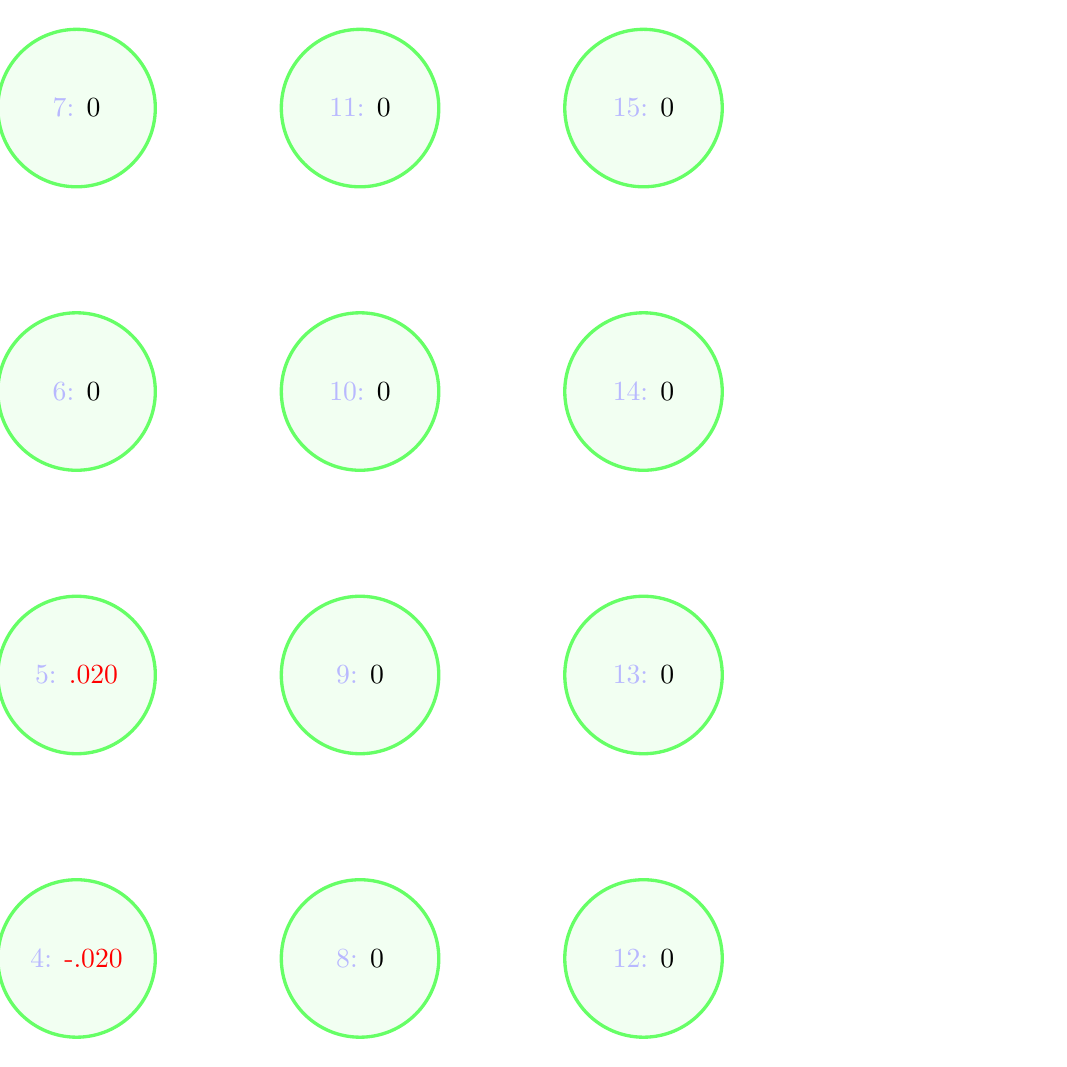
\begin{tikzpicture}[roundnode/.style={circle, draw=green!60, fill=green!5, very thick, minimum size=7mm}, scale=1.2]
\hspace{-4cm}

\node[roundnode, minimum size = 2cm] at (0.0, 0.0) {\textcolor{blue!28}{0:} \textcolor{red}{.040}};
\node[roundnode, minimum size = 2cm] at (0.0, 3.0) {\textcolor{blue!28}{1:} \textcolor{red}{-.060}};
\node[roundnode, minimum size = 2cm] at (0.0, 6.0) {\textcolor{blue!28}{2:} \textcolor{red}{.020}};
\node[roundnode, minimum size = 2cm] at (0.0, 9.0) {\textcolor{blue!28}{3:} 0};
\node[roundnode, minimum size = 2cm] at (3.0, 0.0) {\textcolor{blue!28}{4:} \textcolor{red}{-.020}};
\node[roundnode, minimum size = 2cm] at (3.0, 3.0) {\textcolor{blue!28}{5:} \textcolor{red}{.020}};
\node[roundnode, minimum size = 2cm] at (3.0, 6.0) {\textcolor{blue!28}{6:} 0};
\node[roundnode, minimum size = 2cm] at (3.0, 9.0) {\textcolor{blue!28}{7:} 0};
\node[roundnode, minimum size = 2cm] at (6.0, 0.0) {\textcolor{blue!28}{8:} 0};
\node[roundnode, minimum size = 2cm] at (6.0, 3.0) {\textcolor{blue!28}{9:} 0};
\node[roundnode, minimum size = 2cm] at (6.0, 6.0) {\textcolor{blue!28}{10:} 0};
\node[roundnode, minimum size = 2cm] at (6.0, 9.0) {\textcolor{blue!28}{11:} 0};
\node[roundnode, minimum size = 2cm] at (9.0, 0.0) {\textcolor{blue!28}{12:} 0};
\node[roundnode, minimum size = 2cm] at (9.0, 3.0) {\textcolor{blue!28}{13:} 0};
\node[roundnode, minimum size = 2cm] at (9.0, 6.0) {\textcolor{blue!28}{14:} 0};
\node[roundnode, minimum size = 2cm] at (9.0, 9.0) {\textcolor{blue!28}{15:} 0};

\end{tikzpicture}

\newpage
\section{Gradient Calculation}
\subsection{Given Flow}
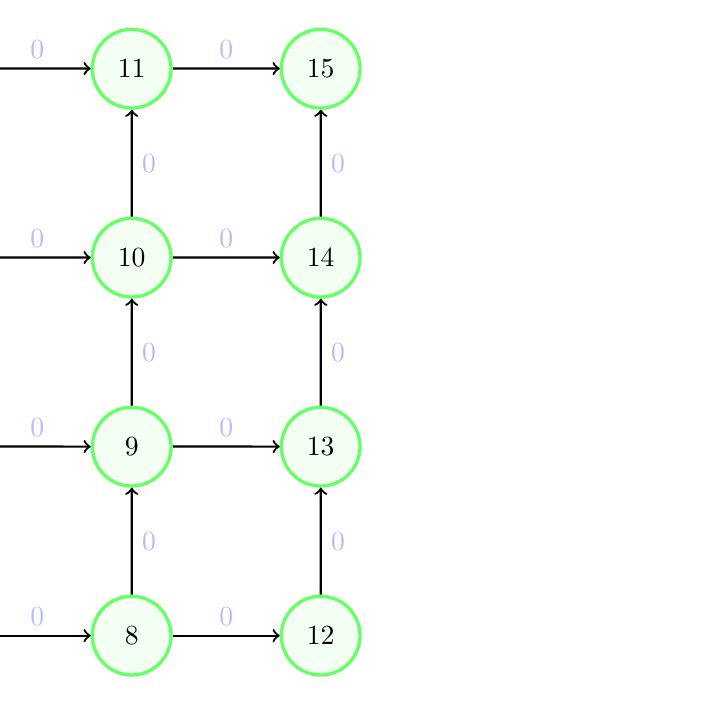
\begin{tikzpicture}[roundnode/.style={circle, draw=green!60, fill=green!5, very thick, minimum size=7mm}, scale=1.2]
\hspace{-4cm}

\node[roundnode, minimum size = 1cm] at (0.0, 0.0) (0) {\textcolor{black}{0}};
\node[roundnode, minimum size = 1cm] at (0.0, 2.0) (1) {\textcolor{black}{1}};
\node[roundnode, minimum size = 1cm] at (0.0, 4.0) (2) {\textcolor{black}{2}};
\node[roundnode, minimum size = 1cm] at (0.0, 6.0) (3) {\textcolor{black}{3}};
\node[roundnode, minimum size = 1cm] at (2.0, 0.0) (4) {\textcolor{black}{4}};
\node[roundnode, minimum size = 1cm] at (2.0, 2.0) (5) {\textcolor{black}{5}};
\node[roundnode, minimum size = 1cm] at (2.0, 4.0) (6) {\textcolor{black}{6}};
\node[roundnode, minimum size = 1cm] at (2.0, 6.0) (7) {\textcolor{black}{7}};
\node[roundnode, minimum size = 1cm] at (4.0, 0.0) (8) {\textcolor{black}{8}};
\node[roundnode, minimum size = 1cm] at (4.0, 2.0) (9) {\textcolor{black}{9}};
\node[roundnode, minimum size = 1cm] at (4.0, 4.0) (10) {\textcolor{black}{10}};
\node[roundnode, minimum size = 1cm] at (4.0, 6.0) (11) {\textcolor{black}{11}};
\node[roundnode, minimum size = 1cm] at (6.0, 0.0) (12) {\textcolor{black}{12}};
\node[roundnode, minimum size = 1cm] at (6.0, 2.0) (13) {\textcolor{black}{13}};
\node[roundnode, minimum size = 1cm] at (6.0, 4.0) (14) {\textcolor{black}{14}};
\node[roundnode, minimum size = 1cm] at (6.0, 6.0) (15) {\textcolor{black}{15}};
\draw[thick, ->] (0) -- (4) node[midway,above] {\textcolor{blue!28}{0}};
\draw[thick, ->] (0) -- (1) node[midway,right] {\textcolor{blue!28}{0}};
\draw[thick, ->] (1) -- (5) node[midway,above] {\textcolor{blue!28}{0}};
\draw[thick, ->] (1) -- (2) node[midway,right] {\textcolor{blue!28}{0}};
\draw[thick, ->] (2) -- (6) node[midway,above] {\textcolor{blue!28}{0}};
\draw[thick, ->] (2) -- (3) node[midway,right] {\textcolor{blue!28}{0}};
\draw[thick, ->] (3) -- (7) node[midway,above] {\textcolor{blue!28}{0}};
\draw[thick, ->] (4) -- (8) node[midway,above] {\textcolor{blue!28}{0}};
\draw[thick, ->] (4) -- (5) node[midway,right] {\textcolor{blue!28}{0}};
\draw[thick, ->] (5) -- (9) node[midway,above] {\textcolor{blue!28}{0}};
\draw[thick, ->] (5) -- (6) node[midway,right] {\textcolor{blue!28}{0}};
\draw[thick, ->] (6) -- (10) node[midway,above] {\textcolor{blue!28}{0}};
\draw[thick, ->] (6) -- (7) node[midway,right] {\textcolor{blue!28}{0}};
\draw[thick, ->] (7) -- (11) node[midway,above] {\textcolor{blue!28}{0}};
\draw[thick, ->] (8) -- (12) node[midway,above] {\textcolor{blue!28}{0}};
\draw[thick, ->] (8) -- (9) node[midway,right] {\textcolor{blue!28}{0}};
\draw[thick, ->] (9) -- (13) node[midway,above] {\textcolor{blue!28}{0}};
\draw[thick, ->] (9) -- (10) node[midway,right] {\textcolor{blue!28}{0}};
\draw[thick, ->] (10) -- (14) node[midway,above] {\textcolor{blue!28}{0}};
\draw[thick, ->] (10) -- (11) node[midway,right] {\textcolor{blue!28}{0}};
\draw[thick, ->] (11) -- (15) node[midway,above] {\textcolor{blue!28}{0}};
\draw[thick, ->] (12) -- (13) node[midway,right] {\textcolor{blue!28}{0}};
\draw[thick, ->] (13) -- (14) node[midway,right] {\textcolor{blue!28}{0}};
\draw[thick, ->] (14) -- (15) node[midway,right] {\textcolor{blue!28}{0}};

\end{tikzpicture}
\subsection{Given Demand}
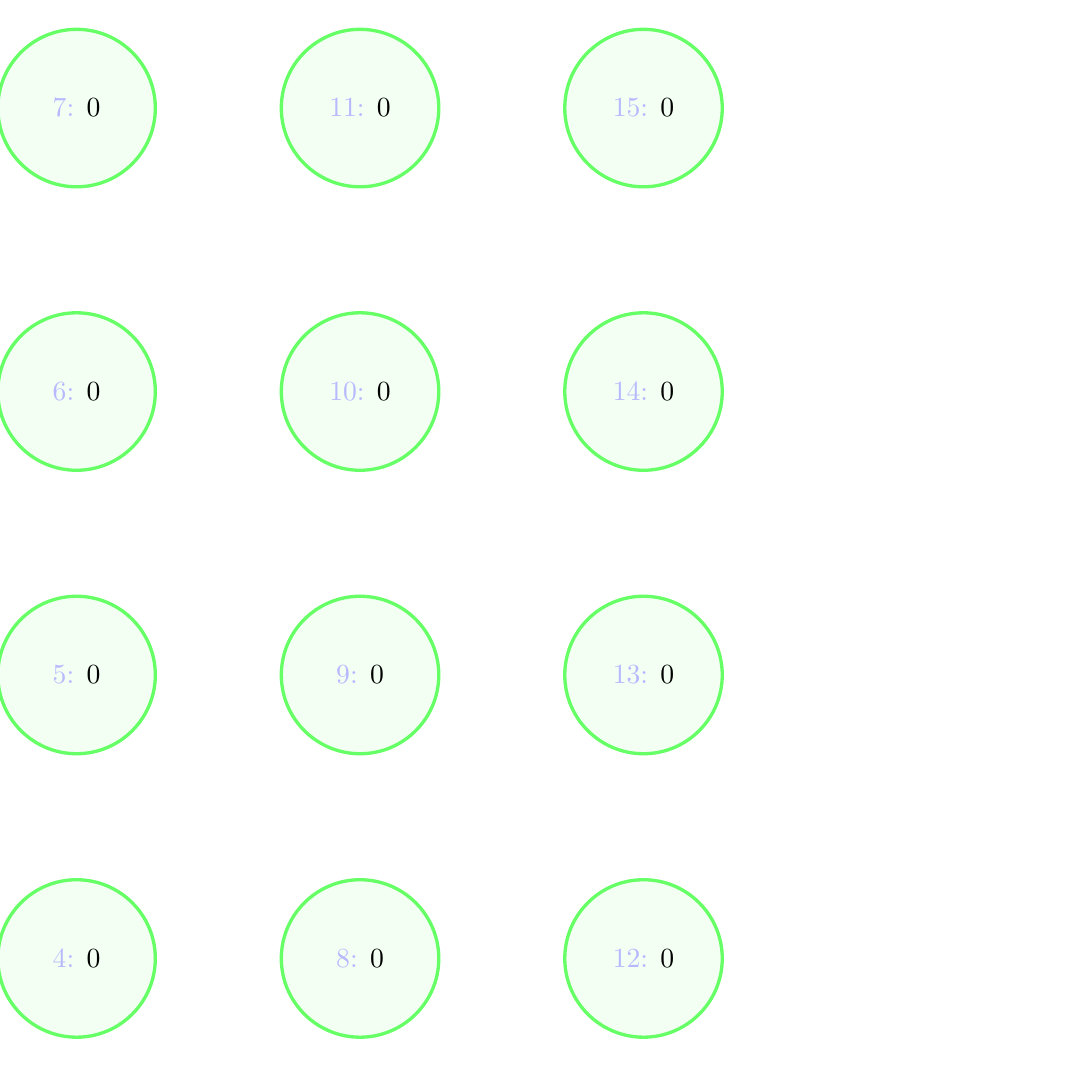
\begin{tikzpicture}[roundnode/.style={circle, draw=green!60, fill=green!5, very thick, minimum size=7mm}, scale=1.2]
\hspace{-4cm}

\node[roundnode, minimum size = 2cm] at (0.0, 0.0) {\textcolor{blue!28}{0:} \textcolor{red}{-8.872}};
\node[roundnode, minimum size = 2cm] at (0.0, 3.0) {\textcolor{blue!28}{1:} \textcolor{red}{8.872}};
\node[roundnode, minimum size = 2cm] at (0.0, 6.0) {\textcolor{blue!28}{2:} 0};
\node[roundnode, minimum size = 2cm] at (0.0, 9.0) {\textcolor{blue!28}{3:} 0};
\node[roundnode, minimum size = 2cm] at (3.0, 0.0) {\textcolor{blue!28}{4:} 0};
\node[roundnode, minimum size = 2cm] at (3.0, 3.0) {\textcolor{blue!28}{5:} 0};
\node[roundnode, minimum size = 2cm] at (3.0, 6.0) {\textcolor{blue!28}{6:} 0};
\node[roundnode, minimum size = 2cm] at (3.0, 9.0) {\textcolor{blue!28}{7:} 0};
\node[roundnode, minimum size = 2cm] at (6.0, 0.0) {\textcolor{blue!28}{8:} 0};
\node[roundnode, minimum size = 2cm] at (6.0, 3.0) {\textcolor{blue!28}{9:} 0};
\node[roundnode, minimum size = 2cm] at (6.0, 6.0) {\textcolor{blue!28}{10:} 0};
\node[roundnode, minimum size = 2cm] at (6.0, 9.0) {\textcolor{blue!28}{11:} 0};
\node[roundnode, minimum size = 2cm] at (9.0, 0.0) {\textcolor{blue!28}{12:} 0};
\node[roundnode, minimum size = 2cm] at (9.0, 3.0) {\textcolor{blue!28}{13:} 0};
\node[roundnode, minimum size = 2cm] at (9.0, 6.0) {\textcolor{blue!28}{14:} 0};
\node[roundnode, minimum size = 2cm] at (9.0, 9.0) {\textcolor{blue!28}{15:} 0};

\end{tikzpicture}
\subsection{Gradient (Graph)}
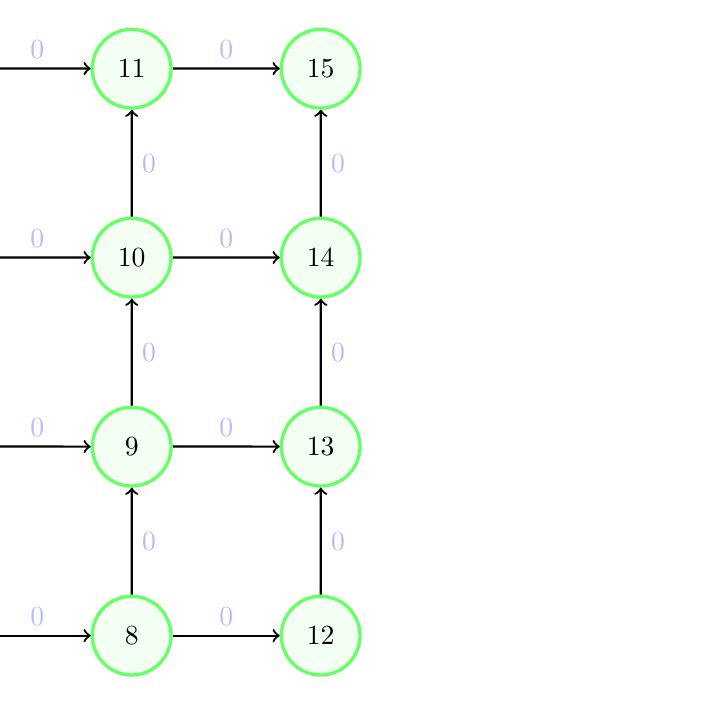
\begin{tikzpicture}[roundnode/.style={circle, draw=green!60, fill=green!5, very thick, minimum size=7mm}, scale=1.2]
\hspace{-4cm}

\node[roundnode, minimum size = 1cm] at (0.0, 0.0) (0) {\textcolor{black}{0}};
\node[roundnode, minimum size = 1cm] at (0.0, 2.0) (1) {\textcolor{black}{1}};
\node[roundnode, minimum size = 1cm] at (0.0, 4.0) (2) {\textcolor{black}{2}};
\node[roundnode, minimum size = 1cm] at (0.0, 6.0) (3) {\textcolor{black}{3}};
\node[roundnode, minimum size = 1cm] at (2.0, 0.0) (4) {\textcolor{black}{4}};
\node[roundnode, minimum size = 1cm] at (2.0, 2.0) (5) {\textcolor{black}{5}};
\node[roundnode, minimum size = 1cm] at (2.0, 4.0) (6) {\textcolor{black}{6}};
\node[roundnode, minimum size = 1cm] at (2.0, 6.0) (7) {\textcolor{black}{7}};
\node[roundnode, minimum size = 1cm] at (4.0, 0.0) (8) {\textcolor{black}{8}};
\node[roundnode, minimum size = 1cm] at (4.0, 2.0) (9) {\textcolor{black}{9}};
\node[roundnode, minimum size = 1cm] at (4.0, 4.0) (10) {\textcolor{black}{10}};
\node[roundnode, minimum size = 1cm] at (4.0, 6.0) (11) {\textcolor{black}{11}};
\node[roundnode, minimum size = 1cm] at (6.0, 0.0) (12) {\textcolor{black}{12}};
\node[roundnode, minimum size = 1cm] at (6.0, 2.0) (13) {\textcolor{black}{13}};
\node[roundnode, minimum size = 1cm] at (6.0, 4.0) (14) {\textcolor{black}{14}};
\node[roundnode, minimum size = 1cm] at (6.0, 6.0) (15) {\textcolor{black}{15}};
\draw[thick, ->] (0) -- (4) node[midway,above] {\textcolor{blue!28}{0}};
\draw[thick, ->] (0) -- (1) node[midway,right] {\textcolor{blue!28}{0}};
\draw[thick, ->] (1) -- (5) node[midway,above] {\textcolor{blue!28}{0}};
\draw[thick, ->] (1) -- (2) node[midway,right] {\textcolor{blue!28}{0}};
\draw[thick, ->] (2) -- (6) node[midway,above] {\textcolor{blue!28}{0}};
\draw[thick, ->] (2) -- (3) node[midway,right] {\textcolor{blue!28}{0}};
\draw[thick, ->] (3) -- (7) node[midway,above] {\textcolor{blue!28}{0}};
\draw[thick, ->] (4) -- (8) node[midway,above] {\textcolor{blue!28}{0}};
\draw[thick, ->] (4) -- (5) node[midway,right] {\textcolor{blue!28}{0}};
\draw[thick, ->] (5) -- (9) node[midway,above] {\textcolor{blue!28}{0}};
\draw[thick, ->] (5) -- (6) node[midway,right] {\textcolor{blue!28}{0}};
\draw[thick, ->] (6) -- (10) node[midway,above] {\textcolor{blue!28}{0}};
\draw[thick, ->] (6) -- (7) node[midway,right] {\textcolor{blue!28}{0}};
\draw[thick, ->] (7) -- (11) node[midway,above] {\textcolor{blue!28}{0}};
\draw[thick, ->] (8) -- (12) node[midway,above] {\textcolor{blue!28}{0}};
\draw[thick, ->] (8) -- (9) node[midway,right] {\textcolor{blue!28}{0}};
\draw[thick, ->] (9) -- (13) node[midway,above] {\textcolor{blue!28}{0}};
\draw[thick, ->] (9) -- (10) node[midway,right] {\textcolor{blue!28}{0}};
\draw[thick, ->] (10) -- (14) node[midway,above] {\textcolor{blue!28}{0}};
\draw[thick, ->] (10) -- (11) node[midway,right] {\textcolor{blue!28}{0}};
\draw[thick, ->] (11) -- (15) node[midway,above] {\textcolor{blue!28}{0}};
\draw[thick, ->] (12) -- (13) node[midway,right] {\textcolor{blue!28}{0}};
\draw[thick, ->] (13) -- (14) node[midway,right] {\textcolor{blue!28}{0}};
\draw[thick, ->] (14) -- (15) node[midway,right] {\textcolor{blue!28}{0}};

\end{tikzpicture}
\subsection{Current Tree}
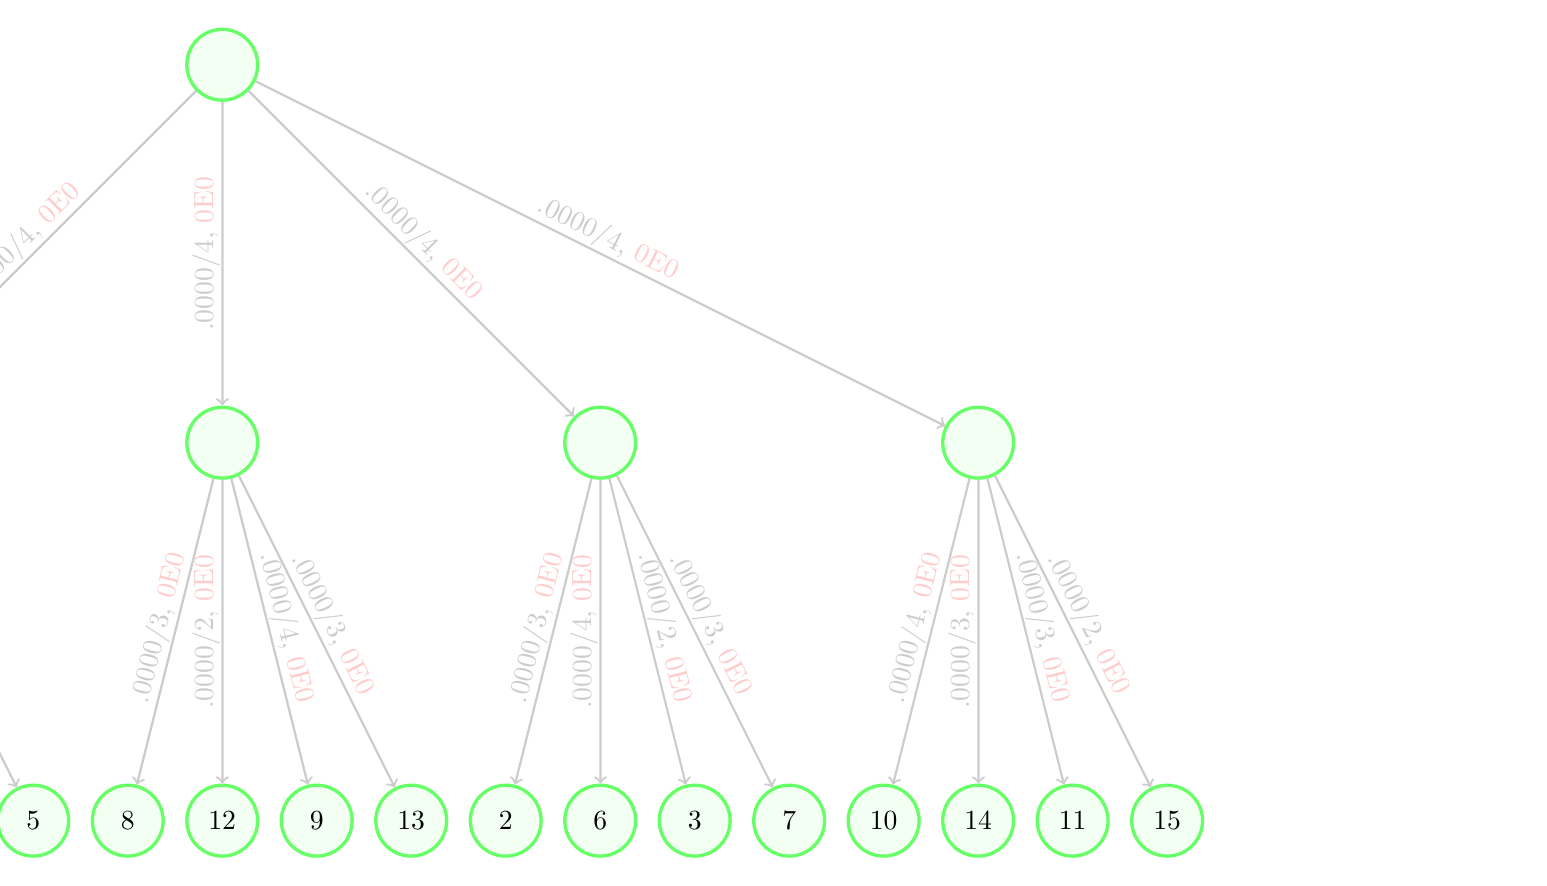
\begin{tikzpicture}[roundnode/.style={circle, draw=green!60, fill=green!5, very thick, minimum size=7mm}, scale=1.2]
\hspace{-4cm}

\node[roundnode, minimum size = 0.9cm] at (8.0, 8) (0h8) {};
\node[roundnode, minimum size = 0.9cm] at (4.0, 4) (2h4) {};
\node[roundnode, minimum size = 0.9cm] at (3.0, 0) (2h0) {0};
\draw[thick, ->, color=blue!40] (2h4) -- (2h0) node[sloped,midway,above=-0.1cm] {\textcolor{black}{-8.8723/2}, \textcolor{red}{-1E0}};
\node[roundnode, minimum size = 0.9cm] at (4.0, 0) (3h0) {4};
\draw[thick, ->, color=black!20] (2h4) -- (3h0) node[sloped,midway,above=-0.1cm] {\textcolor{black!20}{.0000/3}, \textcolor{red!20}{0E0}};
\node[roundnode, minimum size = 0.9cm] at (5.0, 0) (4h0) {1};
\draw[thick, ->, color=blue!40] (2h4) -- (4h0) node[sloped,midway,above=-0.1cm] {\textcolor{black}{8.8723/3}, \textcolor{red}{60.29E-66}};
\node[roundnode, minimum size = 0.9cm] at (6.0, 0) (5h0) {5};
\draw[thick, ->, color=black!20] (2h4) -- (5h0) node[sloped,midway,above=-0.1cm] {\textcolor{black!20}{.0000/4}, \textcolor{red!20}{0E0}};
\draw[thick, ->, color=black!20] (0h8) -- (2h4) node[sloped,midway,above=-0.1cm] {\textcolor{black!20}{.0000/4}, \textcolor{red!20}{0E0}};
\node[roundnode, minimum size = 0.9cm] at (8.0, 4) (6h4) {};
\node[roundnode, minimum size = 0.9cm] at (7.0, 0) (6h0) {8};
\draw[thick, ->, color=black!20] (6h4) -- (6h0) node[sloped,midway,above=-0.1cm] {\textcolor{black!20}{.0000/3}, \textcolor{red!20}{0E0}};
\node[roundnode, minimum size = 0.9cm] at (8.0, 0) (7h0) {12};
\draw[thick, ->, color=black!20] (6h4) -- (7h0) node[sloped,midway,above=-0.1cm] {\textcolor{black!20}{.0000/2}, \textcolor{red!20}{0E0}};
\node[roundnode, minimum size = 0.9cm] at (9.0, 0) (8h0) {9};
\draw[thick, ->, color=black!20] (6h4) -- (8h0) node[sloped,midway,above=-0.1cm] {\textcolor{black!20}{.0000/4}, \textcolor{red!20}{0E0}};
\node[roundnode, minimum size = 0.9cm] at (10.0, 0) (9h0) {13};
\draw[thick, ->, color=black!20] (6h4) -- (9h0) node[sloped,midway,above=-0.1cm] {\textcolor{black!20}{.0000/3}, \textcolor{red!20}{0E0}};
\draw[thick, ->, color=black!20] (0h8) -- (6h4) node[sloped,midway,above=-0.1cm] {\textcolor{black!20}{.0000/4}, \textcolor{red!20}{0E0}};
\node[roundnode, minimum size = 0.9cm] at (12.0, 4) (10h4) {};
\node[roundnode, minimum size = 0.9cm] at (11.0, 0) (10h0) {2};
\draw[thick, ->, color=black!20] (10h4) -- (10h0) node[sloped,midway,above=-0.1cm] {\textcolor{black!20}{.0000/3}, \textcolor{red!20}{0E0}};
\node[roundnode, minimum size = 0.9cm] at (12.0, 0) (11h0) {6};
\draw[thick, ->, color=black!20] (10h4) -- (11h0) node[sloped,midway,above=-0.1cm] {\textcolor{black!20}{.0000/4}, \textcolor{red!20}{0E0}};
\node[roundnode, minimum size = 0.9cm] at (13.0, 0) (12h0) {3};
\draw[thick, ->, color=black!20] (10h4) -- (12h0) node[sloped,midway,above=-0.1cm] {\textcolor{black!20}{.0000/2}, \textcolor{red!20}{0E0}};
\node[roundnode, minimum size = 0.9cm] at (14.0, 0) (13h0) {7};
\draw[thick, ->, color=black!20] (10h4) -- (13h0) node[sloped,midway,above=-0.1cm] {\textcolor{black!20}{.0000/3}, \textcolor{red!20}{0E0}};
\draw[thick, ->, color=black!20] (0h8) -- (10h4) node[sloped,midway,above=-0.1cm] {\textcolor{black!20}{.0000/4}, \textcolor{red!20}{0E0}};
\node[roundnode, minimum size = 0.9cm] at (16.0, 4) (14h4) {};
\node[roundnode, minimum size = 0.9cm] at (15.0, 0) (14h0) {10};
\draw[thick, ->, color=black!20] (14h4) -- (14h0) node[sloped,midway,above=-0.1cm] {\textcolor{black!20}{.0000/4}, \textcolor{red!20}{0E0}};
\node[roundnode, minimum size = 0.9cm] at (16.0, 0) (15h0) {14};
\draw[thick, ->, color=black!20] (14h4) -- (15h0) node[sloped,midway,above=-0.1cm] {\textcolor{black!20}{.0000/3}, \textcolor{red!20}{0E0}};
\node[roundnode, minimum size = 0.9cm] at (17.0, 0) (16h0) {11};
\draw[thick, ->, color=black!20] (14h4) -- (16h0) node[sloped,midway,above=-0.1cm] {\textcolor{black!20}{.0000/3}, \textcolor{red!20}{0E0}};
\node[roundnode, minimum size = 0.9cm] at (18.0, 0) (17h0) {15};
\draw[thick, ->, color=black!20] (14h4) -- (17h0) node[sloped,midway,above=-0.1cm] {\textcolor{black!20}{.0000/2}, \textcolor{red!20}{0E0}};
\draw[thick, ->, color=black!20] (0h8) -- (14h4) node[sloped,midway,above=-0.1cm] {\textcolor{black!20}{.0000/4}, \textcolor{red!20}{0E0}};

\end{tikzpicture}
\subsection{$R^T\cdot \nabla \text{lmax}$}
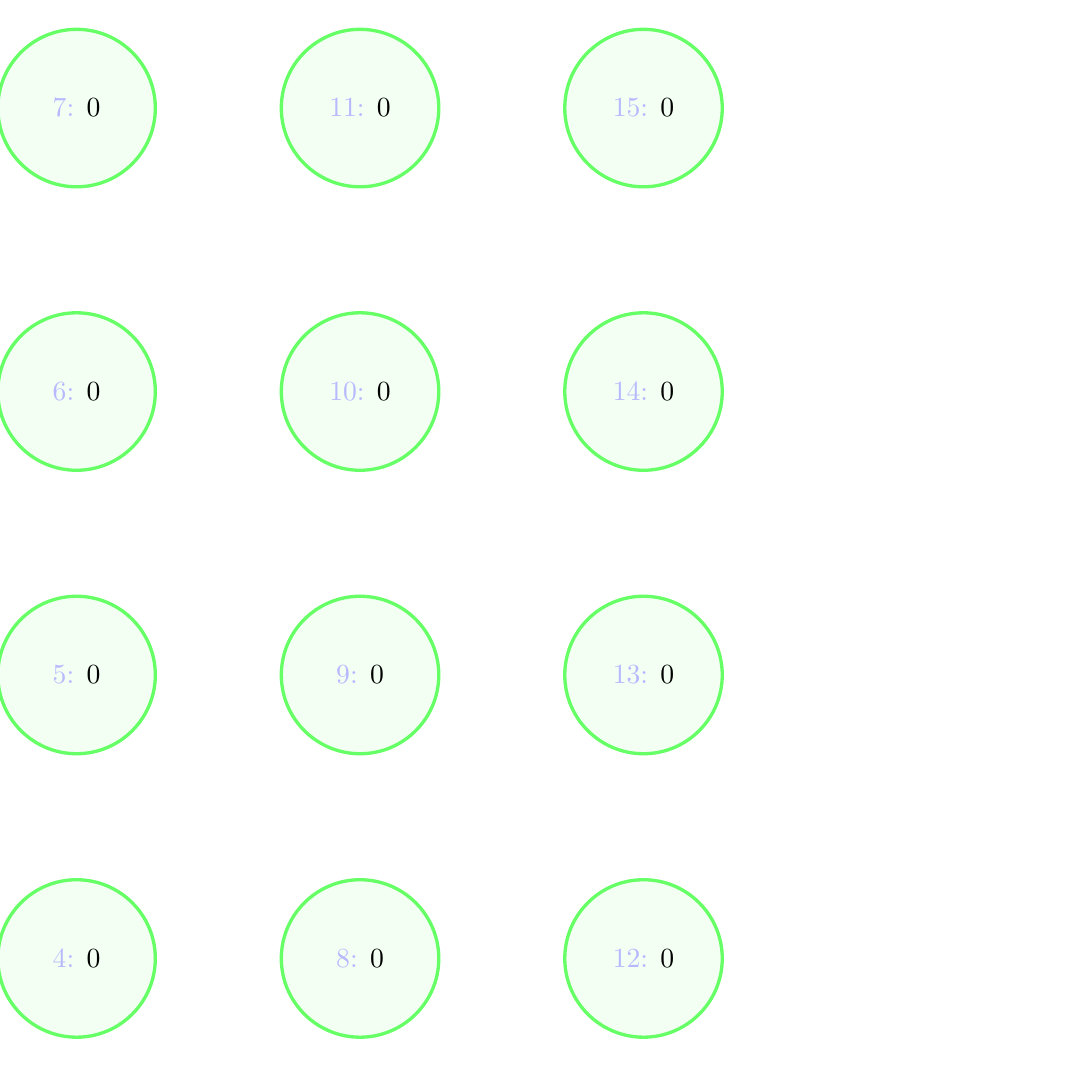
\begin{tikzpicture}[roundnode/.style={circle, draw=green!60, fill=green!5, very thick, minimum size=7mm}, scale=1.2]
\hspace{-4cm}

\node[roundnode, minimum size = 2cm] at (0.0, 0.0) {\textcolor{blue!28}{0:} \textcolor{red}{-1.000}};
\node[roundnode, minimum size = 2cm] at (0.0, 3.0) {\textcolor{blue!28}{1:} \textcolor{red}{.000}};
\node[roundnode, minimum size = 2cm] at (0.0, 6.0) {\textcolor{blue!28}{2:} 0};
\node[roundnode, minimum size = 2cm] at (0.0, 9.0) {\textcolor{blue!28}{3:} 0};
\node[roundnode, minimum size = 2cm] at (3.0, 0.0) {\textcolor{blue!28}{4:} 0};
\node[roundnode, minimum size = 2cm] at (3.0, 3.0) {\textcolor{blue!28}{5:} 0};
\node[roundnode, minimum size = 2cm] at (3.0, 6.0) {\textcolor{blue!28}{6:} 0};
\node[roundnode, minimum size = 2cm] at (3.0, 9.0) {\textcolor{blue!28}{7:} 0};
\node[roundnode, minimum size = 2cm] at (6.0, 0.0) {\textcolor{blue!28}{8:} 0};
\node[roundnode, minimum size = 2cm] at (6.0, 3.0) {\textcolor{blue!28}{9:} 0};
\node[roundnode, minimum size = 2cm] at (6.0, 6.0) {\textcolor{blue!28}{10:} 0};
\node[roundnode, minimum size = 2cm] at (6.0, 9.0) {\textcolor{blue!28}{11:} 0};
\node[roundnode, minimum size = 2cm] at (9.0, 0.0) {\textcolor{blue!28}{12:} 0};
\node[roundnode, minimum size = 2cm] at (9.0, 3.0) {\textcolor{blue!28}{13:} 0};
\node[roundnode, minimum size = 2cm] at (9.0, 6.0) {\textcolor{blue!28}{14:} 0};
\node[roundnode, minimum size = 2cm] at (9.0, 9.0) {\textcolor{blue!28}{15:} 0};

\end{tikzpicture}
\subsection{$B^T \cdot R^T\cdot \nabla \text{lmax}$}
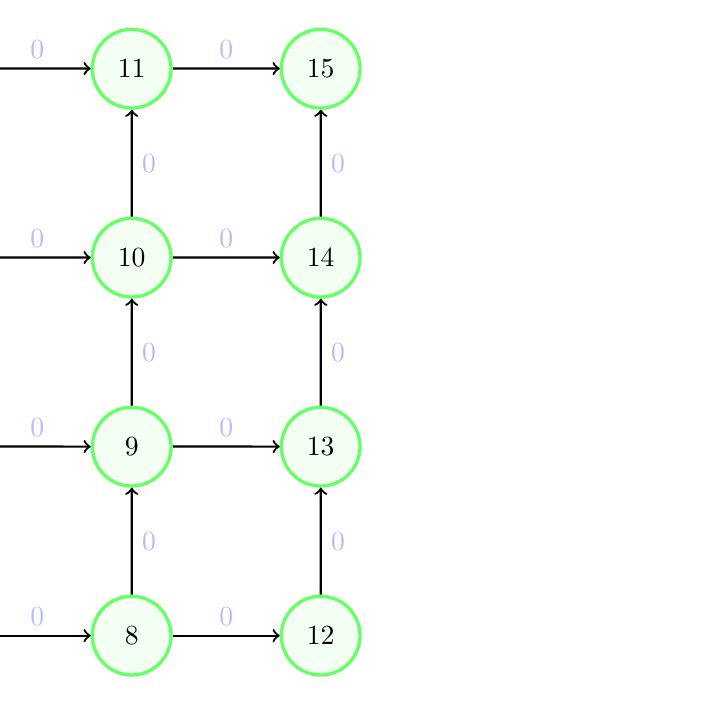
\begin{tikzpicture}[roundnode/.style={circle, draw=green!60, fill=green!5, very thick, minimum size=7mm}, scale=1.2]
\hspace{-4cm}

\node[roundnode, minimum size = 1cm] at (0.0, 0.0) (0) {\textcolor{black}{0}};
\node[roundnode, minimum size = 1cm] at (0.0, 2.0) (1) {\textcolor{black}{1}};
\node[roundnode, minimum size = 1cm] at (0.0, 4.0) (2) {\textcolor{black}{2}};
\node[roundnode, minimum size = 1cm] at (0.0, 6.0) (3) {\textcolor{black}{3}};
\node[roundnode, minimum size = 1cm] at (2.0, 0.0) (4) {\textcolor{black}{4}};
\node[roundnode, minimum size = 1cm] at (2.0, 2.0) (5) {\textcolor{black}{5}};
\node[roundnode, minimum size = 1cm] at (2.0, 4.0) (6) {\textcolor{black}{6}};
\node[roundnode, minimum size = 1cm] at (2.0, 6.0) (7) {\textcolor{black}{7}};
\node[roundnode, minimum size = 1cm] at (4.0, 0.0) (8) {\textcolor{black}{8}};
\node[roundnode, minimum size = 1cm] at (4.0, 2.0) (9) {\textcolor{black}{9}};
\node[roundnode, minimum size = 1cm] at (4.0, 4.0) (10) {\textcolor{black}{10}};
\node[roundnode, minimum size = 1cm] at (4.0, 6.0) (11) {\textcolor{black}{11}};
\node[roundnode, minimum size = 1cm] at (6.0, 0.0) (12) {\textcolor{black}{12}};
\node[roundnode, minimum size = 1cm] at (6.0, 2.0) (13) {\textcolor{black}{13}};
\node[roundnode, minimum size = 1cm] at (6.0, 4.0) (14) {\textcolor{black}{14}};
\node[roundnode, minimum size = 1cm] at (6.0, 6.0) (15) {\textcolor{black}{15}};
\draw[thick, ->] (0) -- (4) node[midway,above] {-1.000};
\draw[thick, ->] (0) -- (1) node[midway,right] {-1.000};
\draw[thick, ->] (1) -- (5) node[midway,above] {.000};
\draw[thick, ->] (1) -- (2) node[midway,right] {.000};
\draw[thick, ->] (2) -- (6) node[midway,above] {\textcolor{blue!28}{0}};
\draw[thick, ->] (2) -- (3) node[midway,right] {\textcolor{blue!28}{0}};
\draw[thick, ->] (3) -- (7) node[midway,above] {\textcolor{blue!28}{0}};
\draw[thick, ->] (4) -- (8) node[midway,above] {\textcolor{blue!28}{0}};
\draw[thick, ->] (4) -- (5) node[midway,right] {\textcolor{blue!28}{0}};
\draw[thick, ->] (5) -- (9) node[midway,above] {\textcolor{blue!28}{0}};
\draw[thick, ->] (5) -- (6) node[midway,right] {\textcolor{blue!28}{0}};
\draw[thick, ->] (6) -- (10) node[midway,above] {\textcolor{blue!28}{0}};
\draw[thick, ->] (6) -- (7) node[midway,right] {\textcolor{blue!28}{0}};
\draw[thick, ->] (7) -- (11) node[midway,above] {\textcolor{blue!28}{0}};
\draw[thick, ->] (8) -- (12) node[midway,above] {\textcolor{blue!28}{0}};
\draw[thick, ->] (8) -- (9) node[midway,right] {\textcolor{blue!28}{0}};
\draw[thick, ->] (9) -- (13) node[midway,above] {\textcolor{blue!28}{0}};
\draw[thick, ->] (9) -- (10) node[midway,right] {\textcolor{blue!28}{0}};
\draw[thick, ->] (10) -- (14) node[midway,above] {\textcolor{blue!28}{0}};
\draw[thick, ->] (10) -- (11) node[midway,right] {\textcolor{blue!28}{0}};
\draw[thick, ->] (11) -- (15) node[midway,above] {\textcolor{blue!28}{0}};
\draw[thick, ->] (12) -- (13) node[midway,right] {\textcolor{blue!28}{0}};
\draw[thick, ->] (13) -- (14) node[midway,right] {\textcolor{blue!28}{0}};
\draw[thick, ->] (14) -- (15) node[midway,right] {\textcolor{blue!28}{0}};

\end{tikzpicture}
\subsection{$-2\alpha\cdot \frac{1}{\sum_i e^{(2\alpha\cdot R(b-Bf))_i}+e^{(-2\alpha\cdot R(b-Bf))_i}} \cdot B^T \cdot R^T\cdot \nabla \text{lmax}$}
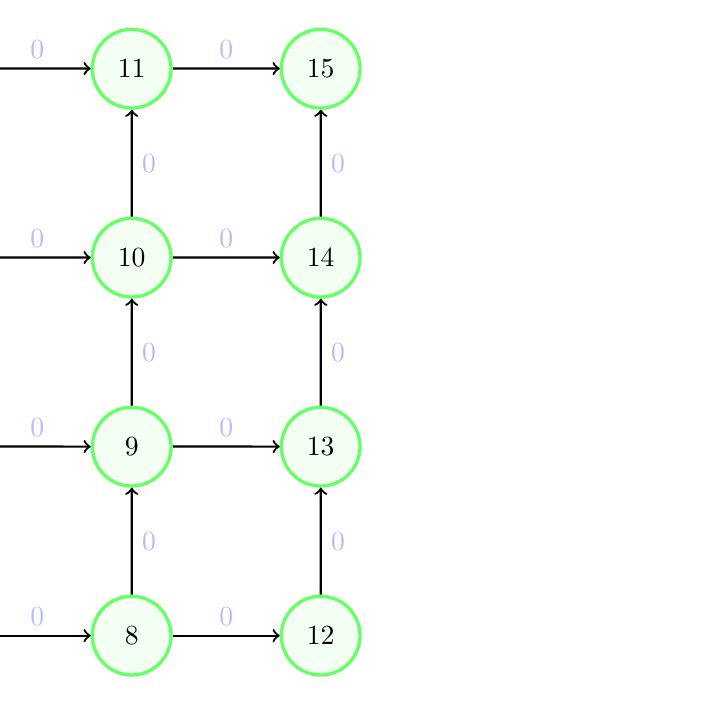
\begin{tikzpicture}[roundnode/.style={circle, draw=green!60, fill=green!5, very thick, minimum size=7mm}, scale=1.2]
\hspace{-4cm}

\node[roundnode, minimum size = 1cm] at (0.0, 0.0) (0) {\textcolor{black}{0}};
\node[roundnode, minimum size = 1cm] at (0.0, 2.0) (1) {\textcolor{black}{1}};
\node[roundnode, minimum size = 1cm] at (0.0, 4.0) (2) {\textcolor{black}{2}};
\node[roundnode, minimum size = 1cm] at (0.0, 6.0) (3) {\textcolor{black}{3}};
\node[roundnode, minimum size = 1cm] at (2.0, 0.0) (4) {\textcolor{black}{4}};
\node[roundnode, minimum size = 1cm] at (2.0, 2.0) (5) {\textcolor{black}{5}};
\node[roundnode, minimum size = 1cm] at (2.0, 4.0) (6) {\textcolor{black}{6}};
\node[roundnode, minimum size = 1cm] at (2.0, 6.0) (7) {\textcolor{black}{7}};
\node[roundnode, minimum size = 1cm] at (4.0, 0.0) (8) {\textcolor{black}{8}};
\node[roundnode, minimum size = 1cm] at (4.0, 2.0) (9) {\textcolor{black}{9}};
\node[roundnode, minimum size = 1cm] at (4.0, 4.0) (10) {\textcolor{black}{10}};
\node[roundnode, minimum size = 1cm] at (4.0, 6.0) (11) {\textcolor{black}{11}};
\node[roundnode, minimum size = 1cm] at (6.0, 0.0) (12) {\textcolor{black}{12}};
\node[roundnode, minimum size = 1cm] at (6.0, 2.0) (13) {\textcolor{black}{13}};
\node[roundnode, minimum size = 1cm] at (6.0, 4.0) (14) {\textcolor{black}{14}};
\node[roundnode, minimum size = 1cm] at (6.0, 6.0) (15) {\textcolor{black}{15}};
\draw[thick, ->] (0) -- (4) node[midway,above] {100.000};
\draw[thick, ->] (0) -- (1) node[midway,right] {100.000};
\draw[thick, ->] (1) -- (5) node[midway,above] {-.000};
\draw[thick, ->] (1) -- (2) node[midway,right] {-.000};
\draw[thick, ->] (2) -- (6) node[midway,above] {\textcolor{blue!28}{0}};
\draw[thick, ->] (2) -- (3) node[midway,right] {\textcolor{blue!28}{0}};
\draw[thick, ->] (3) -- (7) node[midway,above] {\textcolor{blue!28}{0}};
\draw[thick, ->] (4) -- (8) node[midway,above] {\textcolor{blue!28}{0}};
\draw[thick, ->] (4) -- (5) node[midway,right] {\textcolor{blue!28}{0}};
\draw[thick, ->] (5) -- (9) node[midway,above] {\textcolor{blue!28}{0}};
\draw[thick, ->] (5) -- (6) node[midway,right] {\textcolor{blue!28}{0}};
\draw[thick, ->] (6) -- (10) node[midway,above] {\textcolor{blue!28}{0}};
\draw[thick, ->] (6) -- (7) node[midway,right] {\textcolor{blue!28}{0}};
\draw[thick, ->] (7) -- (11) node[midway,above] {\textcolor{blue!28}{0}};
\draw[thick, ->] (8) -- (12) node[midway,above] {\textcolor{blue!28}{0}};
\draw[thick, ->] (8) -- (9) node[midway,right] {\textcolor{blue!28}{0}};
\draw[thick, ->] (9) -- (13) node[midway,above] {\textcolor{blue!28}{0}};
\draw[thick, ->] (9) -- (10) node[midway,right] {\textcolor{blue!28}{0}};
\draw[thick, ->] (10) -- (14) node[midway,above] {\textcolor{blue!28}{0}};
\draw[thick, ->] (10) -- (11) node[midway,right] {\textcolor{blue!28}{0}};
\draw[thick, ->] (11) -- (15) node[midway,above] {\textcolor{blue!28}{0}};
\draw[thick, ->] (12) -- (13) node[midway,right] {\textcolor{blue!28}{0}};
\draw[thick, ->] (13) -- (14) node[midway,right] {\textcolor{blue!28}{0}};
\draw[thick, ->] (14) -- (15) node[midway,right] {\textcolor{blue!28}{0}};

\end{tikzpicture}
\subsection{Total Gradient}
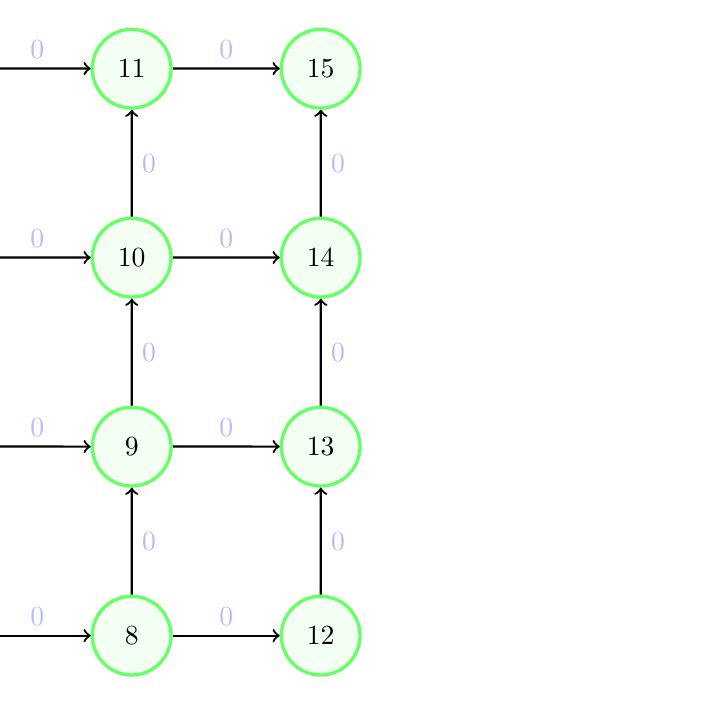
\begin{tikzpicture}[roundnode/.style={circle, draw=green!60, fill=green!5, very thick, minimum size=7mm}, scale=1.2]
\hspace{-4cm}

\node[roundnode, minimum size = 1cm] at (0.0, 0.0) (0) {\textcolor{black}{0}};
\node[roundnode, minimum size = 1cm] at (0.0, 2.0) (1) {\textcolor{black}{1}};
\node[roundnode, minimum size = 1cm] at (0.0, 4.0) (2) {\textcolor{black}{2}};
\node[roundnode, minimum size = 1cm] at (0.0, 6.0) (3) {\textcolor{black}{3}};
\node[roundnode, minimum size = 1cm] at (2.0, 0.0) (4) {\textcolor{black}{4}};
\node[roundnode, minimum size = 1cm] at (2.0, 2.0) (5) {\textcolor{black}{5}};
\node[roundnode, minimum size = 1cm] at (2.0, 4.0) (6) {\textcolor{black}{6}};
\node[roundnode, minimum size = 1cm] at (2.0, 6.0) (7) {\textcolor{black}{7}};
\node[roundnode, minimum size = 1cm] at (4.0, 0.0) (8) {\textcolor{black}{8}};
\node[roundnode, minimum size = 1cm] at (4.0, 2.0) (9) {\textcolor{black}{9}};
\node[roundnode, minimum size = 1cm] at (4.0, 4.0) (10) {\textcolor{black}{10}};
\node[roundnode, minimum size = 1cm] at (4.0, 6.0) (11) {\textcolor{black}{11}};
\node[roundnode, minimum size = 1cm] at (6.0, 0.0) (12) {\textcolor{black}{12}};
\node[roundnode, minimum size = 1cm] at (6.0, 2.0) (13) {\textcolor{black}{13}};
\node[roundnode, minimum size = 1cm] at (6.0, 4.0) (14) {\textcolor{black}{14}};
\node[roundnode, minimum size = 1cm] at (6.0, 6.0) (15) {\textcolor{black}{15}};
\draw[thick, ->] (0) -- (4) node[midway,above] {100.000};
\draw[thick, ->] (0) -- (1) node[midway,right] {100.000};
\draw[thick, ->] (1) -- (5) node[midway,above] {-.000};
\draw[thick, ->] (1) -- (2) node[midway,right] {-.000};
\draw[thick, ->] (2) -- (6) node[midway,above] {\textcolor{blue!28}{0}};
\draw[thick, ->] (2) -- (3) node[midway,right] {\textcolor{blue!28}{0}};
\draw[thick, ->] (3) -- (7) node[midway,above] {\textcolor{blue!28}{0}};
\draw[thick, ->] (4) -- (8) node[midway,above] {\textcolor{blue!28}{0}};
\draw[thick, ->] (4) -- (5) node[midway,right] {\textcolor{blue!28}{0}};
\draw[thick, ->] (5) -- (9) node[midway,above] {\textcolor{blue!28}{0}};
\draw[thick, ->] (5) -- (6) node[midway,right] {\textcolor{blue!28}{0}};
\draw[thick, ->] (6) -- (10) node[midway,above] {\textcolor{blue!28}{0}};
\draw[thick, ->] (6) -- (7) node[midway,right] {\textcolor{blue!28}{0}};
\draw[thick, ->] (7) -- (11) node[midway,above] {\textcolor{blue!28}{0}};
\draw[thick, ->] (8) -- (12) node[midway,above] {\textcolor{blue!28}{0}};
\draw[thick, ->] (8) -- (9) node[midway,right] {\textcolor{blue!28}{0}};
\draw[thick, ->] (9) -- (13) node[midway,above] {\textcolor{blue!28}{0}};
\draw[thick, ->] (9) -- (10) node[midway,right] {\textcolor{blue!28}{0}};
\draw[thick, ->] (10) -- (14) node[midway,above] {\textcolor{blue!28}{0}};
\draw[thick, ->] (10) -- (11) node[midway,right] {\textcolor{blue!28}{0}};
\draw[thick, ->] (11) -- (15) node[midway,above] {\textcolor{blue!28}{0}};
\draw[thick, ->] (12) -- (13) node[midway,right] {\textcolor{blue!28}{0}};
\draw[thick, ->] (13) -- (14) node[midway,right] {\textcolor{blue!28}{0}};
\draw[thick, ->] (14) -- (15) node[midway,right] {\textcolor{blue!28}{0}};

\end{tikzpicture}
\end{document}